\section{Synthesis: comparing the DiVaS and ALoVaS methods}
In this section we compare the DiVaS and ALoVaS. While both methods seem relatively similar, both methods performing variable selection on Bayesian decision trees. There are fundamental practical and theoretical differences between the two methods. 

\subsection{Theoretical differences and a simulation study}

One of the most apparent theoretical differences between the DiVaS and ALoVaS models is the way the two models handle the correlation between covariate selection probabilities. One of the properties of the Dirichlet distribution is that $Corr(p_i,p_j) < 0$ for $i\neq j$. Thus if the prior puts zero probability on non-negative covariant selection probability correlations then the prior will also place zero probability on these non-negative correlations. 

One might be tempted to conclude that this is a element of minut\ae that has no practical consequence but consider a linear model data generating process that contains an interaction between two variables, $x_1$ and $x_2$

\begin{equation}\label{eqn:interaction_model}
y_i = \beta x_1x_2 + \epsilon_i,
\end{equation}  

where $\epsilon_i \sim N(0, \sigma^2$). in this case the coefficient $\beta$ controls the degree of curvature in the $x_1, x_2$ space. The positive covariate selection probability results from using a constant function in each terminal node to approximate a curved two dimensional surface. The constant function requires alternating splits between $x_1$ and $x_2$ to approximate the curving of the $x_1$, $x_2$ space. 

A nice property of the ALoVaS method is that the if $p_i$, $p_j$ be the two covariate selection probabilities, then if these $p_i$, $p_j$ have a logistic normal density the covariance between the two densities is 

\begin{equation}\label{eqn:cov_aln}
Cov(log(p_j/p_k), log(p_l/p_m) ) = \sigma_{jl} + \sigma_{km} - \sigma_{jm} - \sigma_{kl},
\end{equation }

where $\sigma_{ij}$ is the covariance parameter for the normal random variable before the application go the ALT \cite{}. Clearly the four $\sigma_{ij} \geq 0$ in Equation \ref{eqn:cov_aln} so that the covariance could be positive or negative.  

At this point it is worth noting that the idea of an automatic interaction detector was first proposed in the CHAID method \cite{}. The CHAID method claims to automatically detect interactions, yet popular documents \cite{} (cite the sas tree book) claim that CHAID and other decision tree methods cannot actually perform automatic interaction detection. The validity of this claim is not the point of this paragraph but it should be clear to the reader how one could visually inspect a fitted tree and determine if interaction is plausible. Moreover, with the ALoVaS automatic interaction detection is plausible, by comparing the sampled values of $Cov(log(p_j/p_k), log(p_l/p_m) )$  against the point zero one gets an indication of the degree of interaction. Moreover we cannot determine if the interaction is positive or negative, only that an interaction is present. 

\begin{itemize}
\item Correlation of the dirichlet is only negative  
\item Linear models with interactions  
\item A relation with CHAID. Automatic interaction detection is not a myth! 
\item Linear model with a positive interaction between $x_1$ and $x_2$. 
\end{itemize}

We now present a small simulation study. We sampled data according to the model describing in Equation \ref{eqn:interaction_model}. We simulated $n=500$ observations from this model for a training and another for a test, or hold-out data set. We simulated data under the model with $\beta =5, -5$. The trees fitted under a greedy optimization for the two interaction scenarios are shown in Figure \ref{fig:interaction_trees}. 

\begin{figure}
\begin{center} 
\begin{tabular}{cc}
%  \num\putindeepbox[2pt]{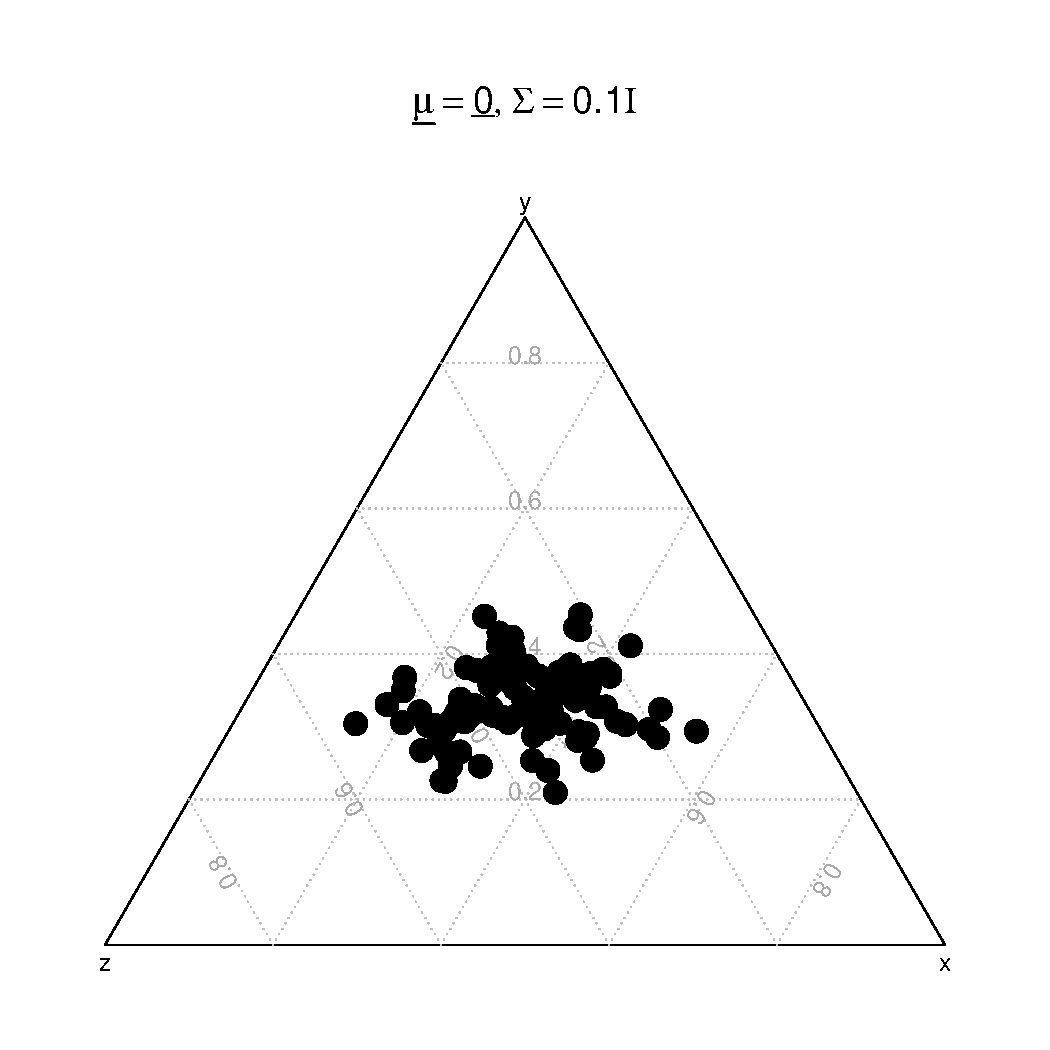
\includegraphics[scale=0.25]{figures/mu0_0_bw.pdf}}
%    & \num\putindeepbox[2pt]{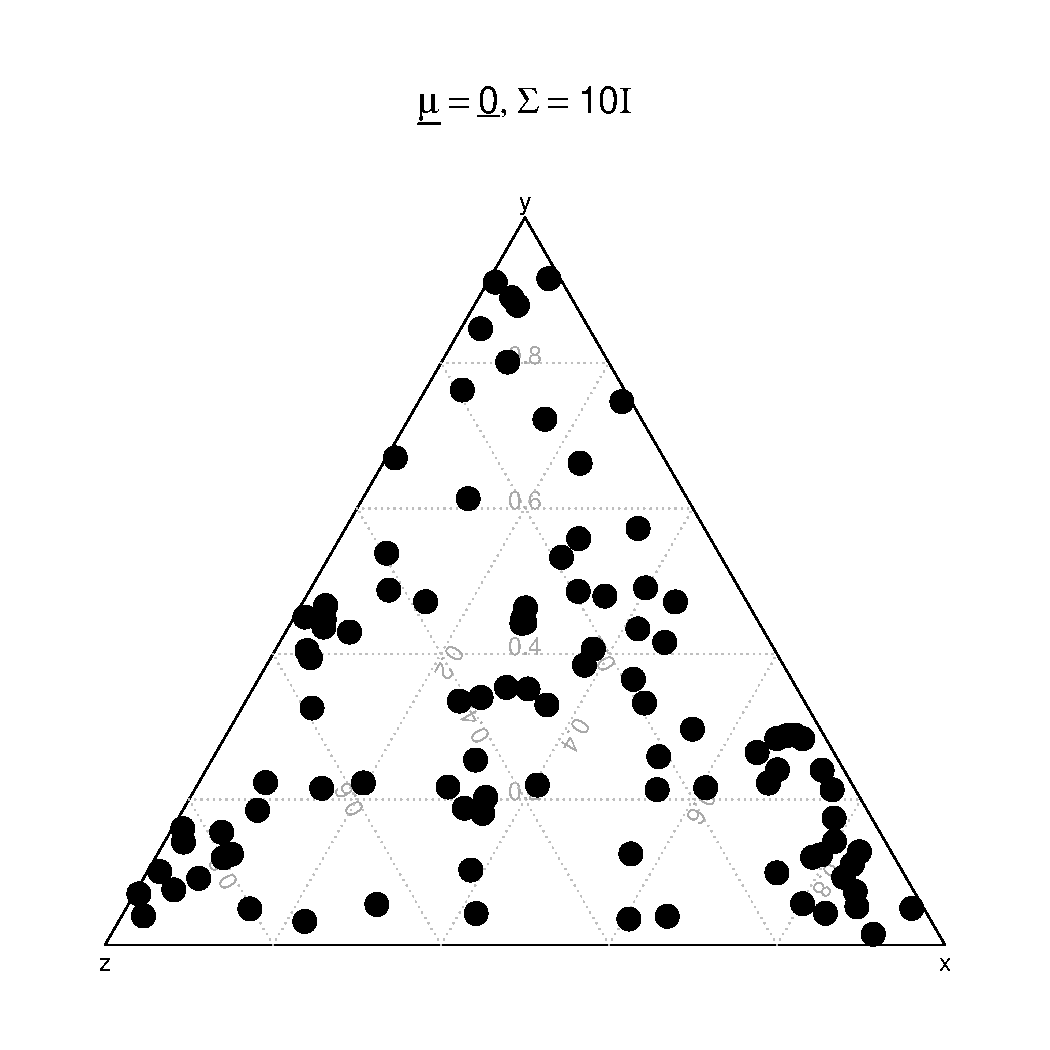
\includegraphics[scale=0.25]{figures/sigma3_3_bw.pdf}} \\
%  \num\putindeepbox[2pt]{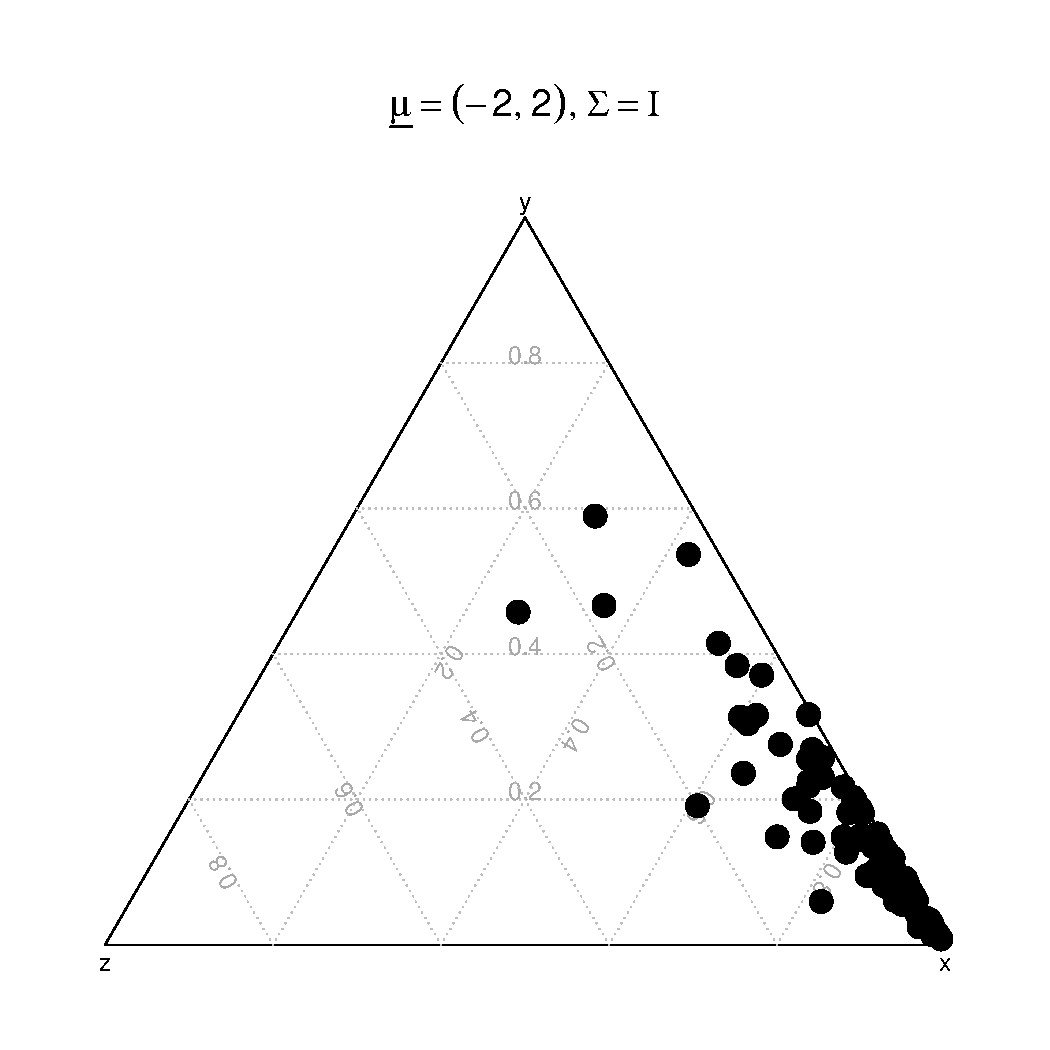
\includegraphics[scale=0.25]{figures/mu2_0_bw.pdf}}
%    & \num\putindeepbox[2pt]{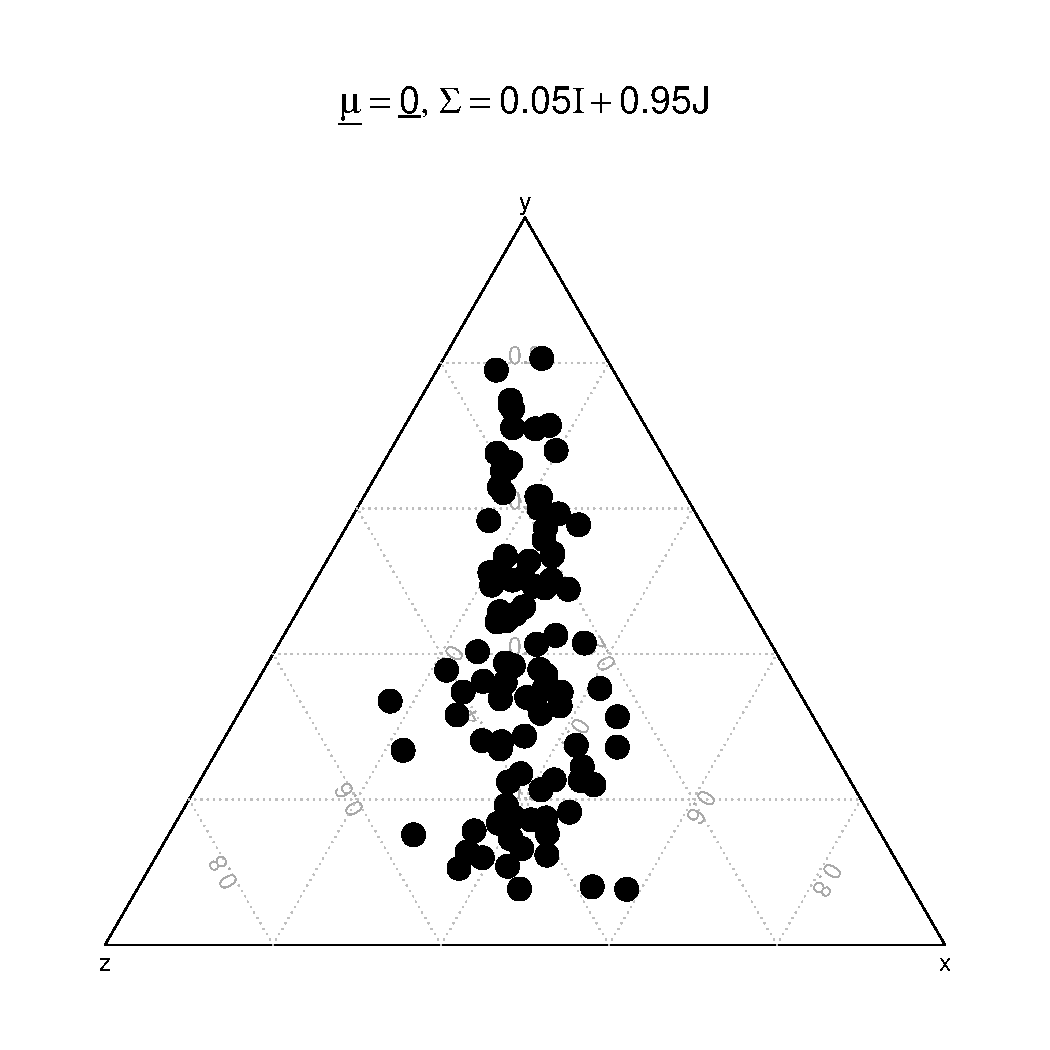
\includegraphics[scale=0.25]{figures/sigma1_9_9_1_bw.pdf}} \\
\end{tabular}
\caption{write the caption here.}
\label{fig:interaction_trees}
\end{center}
\end{figure} 

We ran the ALoVaS and DiVaS algorithms for $10,000$ samples discarding the first $1000$ as a burn-in sample. Convergence statistics were calculated using the coda package in R with Gelman-Rubin statistics of \textbf{blah} and \textbf{blah} for the ALoVaS and DiVaS chains respectively. The trees with the largest integrated likelihood for the two chains are presented in Figure \ref{fig:chain_max_interaction_tree}.  

\begin{figure}
\begin{center} 
\begin{tabular}{cc}
%  \num\putindeepbox[2pt]{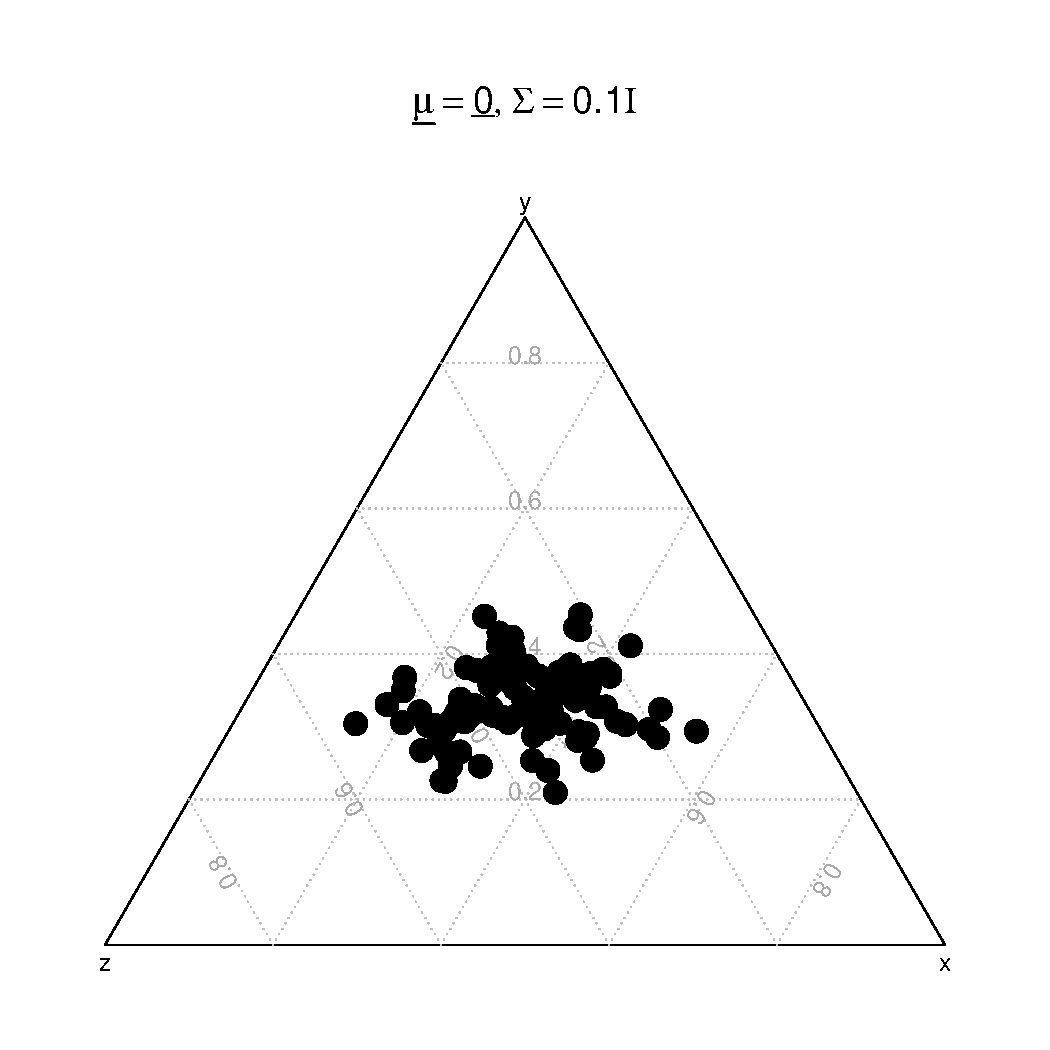
\includegraphics[scale=0.25]{figures/mu0_0_bw.pdf}}
%    & \num\putindeepbox[2pt]{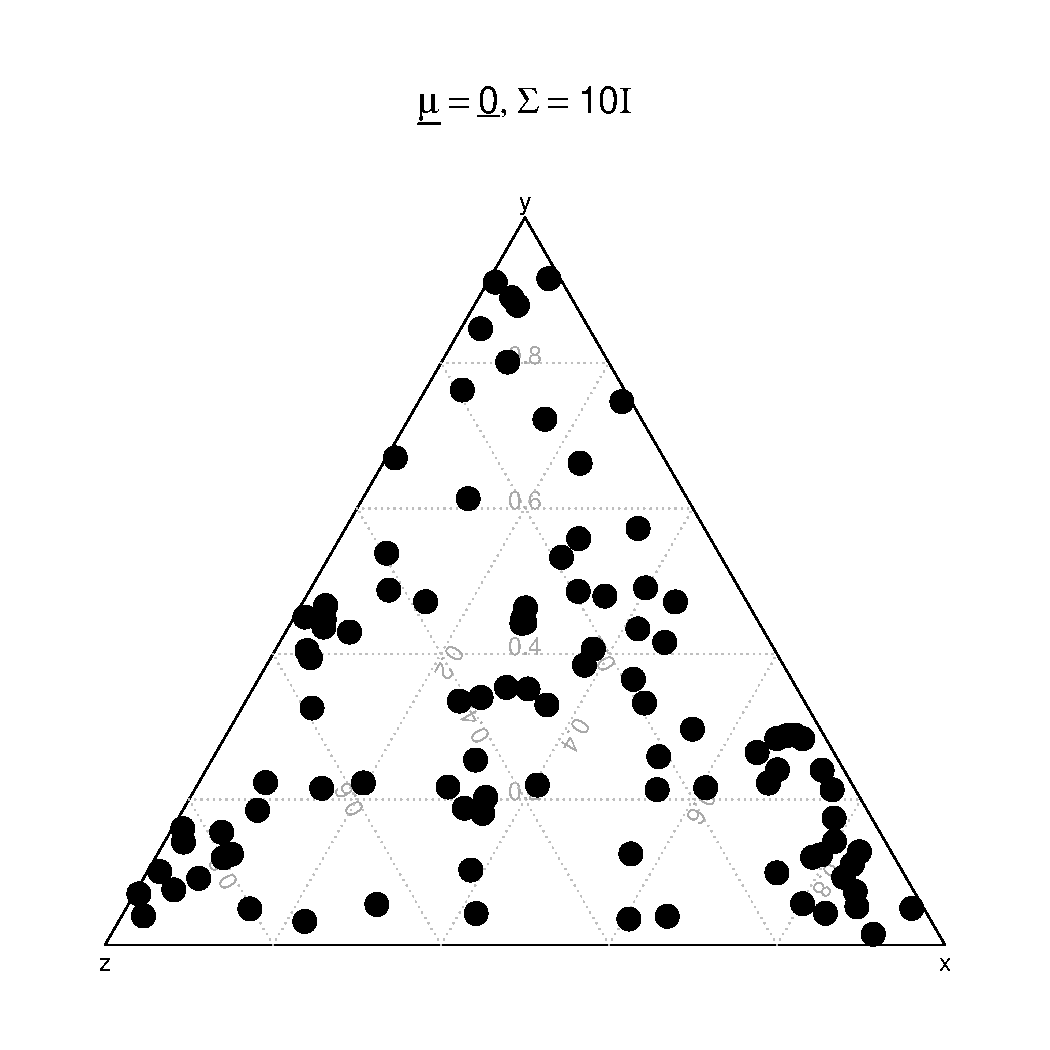
\includegraphics[scale=0.25]{figures/sigma3_3_bw.pdf}} \\
%  \num\putindeepbox[2pt]{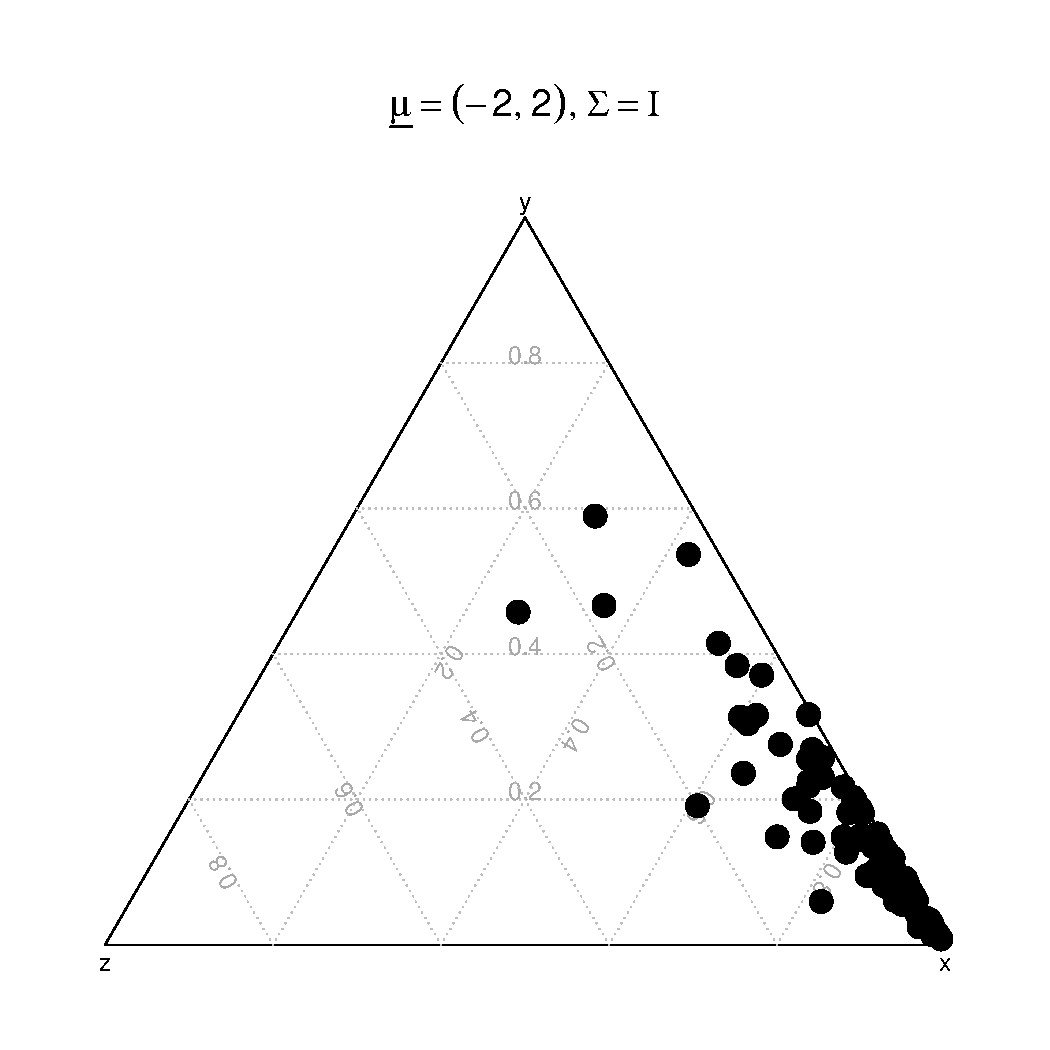
\includegraphics[scale=0.25]{figures/mu2_0_bw.pdf}}
%    & \num\putindeepbox[2pt]{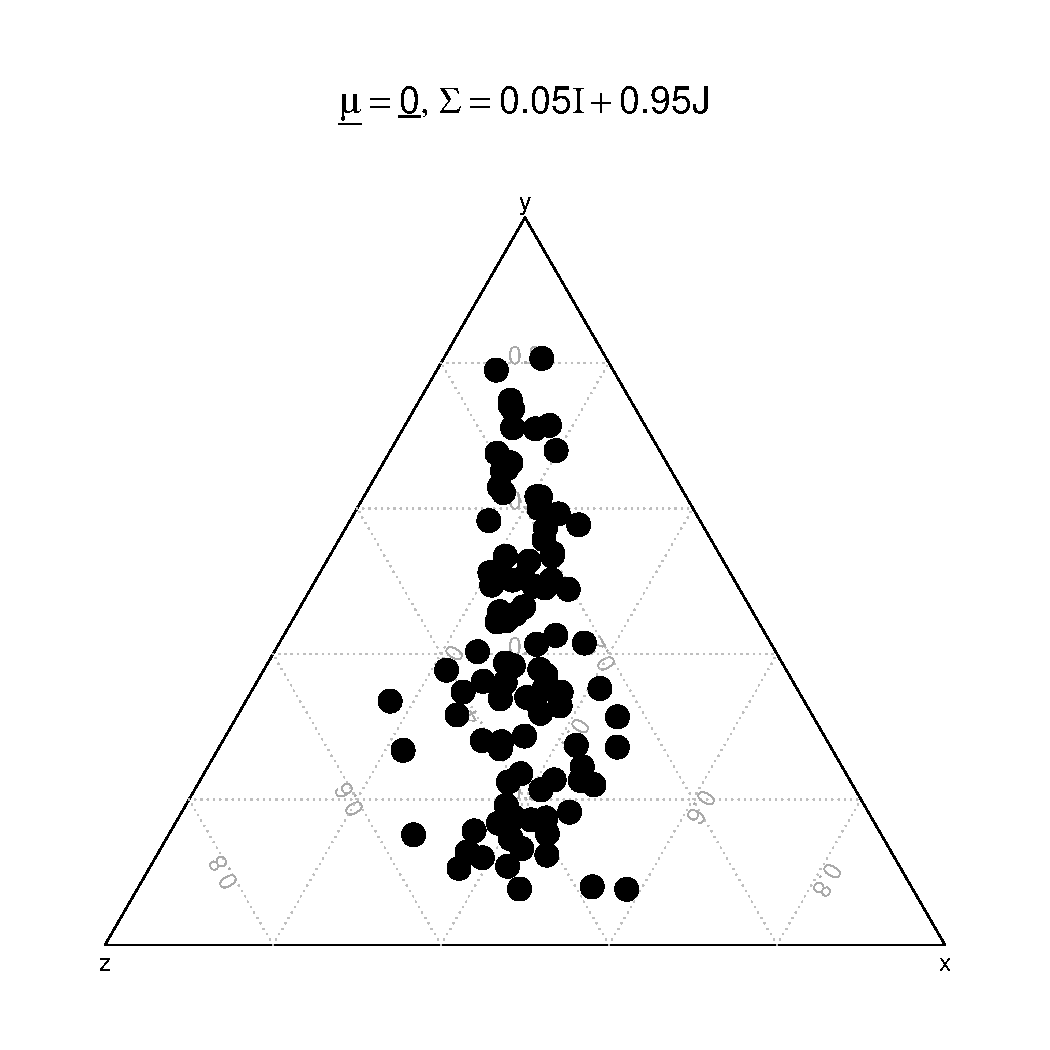
\includegraphics[scale=0.25]{figures/sigma1_9_9_1_bw.pdf}} \\
\end{tabular}
\caption{write the caption here.}
\label{fig:chain_max_interaction_tree}
\end{center}
\end{figure} 

\subsection{Practical differences and a simulation study}

\begin{itemize}
\item Conceptual link between linear models  and decision trees with ALoVaS. 
\item longer to simulate Alovas 
\item DiVaS requires negative correlations, impossible to know \emph{a priori}
\item Positive versus negative correlations, linear models and decision trees
\end{itemize}

\subsection{Conclusions and Recommendations}

\begin{itemize}
\item ALoVaS provides a conceptually simple generic method adaptable to the shrinkage needs of your own problem. 
\item DiVaS is more of an ad-hoc method which can provide promising results. 
\item ALoVaS is to be preferred over DiVaS. 
\end{itemize}

